% ============================================================
% Question Bank: ch09-06 Finding Probabilities of Compound Events
% Topic Title: Finding Probabilities of Compound Events
% CCSS: 7.SP.C.8b
% Questions: 27 (15 MC + 6 SA + 6 Graphical)
% ============================================================

% --- Multiple Choice Questions (15) ---

\begin{practiceQuestion}{9-6-q01}{mc}
\begin{questionText}
A spinner has $4$ equal sections (A, B, C, D) and a coin is flipped. What is the probability of landing on D and getting tails?
\end{questionText}
\choiceA{$\dfrac{1}{2}$}
\choiceB{$\dfrac{1}{4}$}
\choiceC{$\dfrac{1}{6}$}
\choiceD{$\dfrac{1}{8}$}
\correctAnswer{D}
\explanation{The sample space has $4 \times 2 = 8$ equally likely outcomes. Only one outcome is (D, Tails). So $P(\text{D and Tails}) = \frac{1}{8}$.}
\end{practiceQuestion}

\begin{practiceQuestion}{9-6-q02}{mc}
\begin{questionText}
Two standard number cubes are rolled. What is the probability of getting a sum of $5$?
\end{questionText}
\choiceA{$\dfrac{1}{9}$}
\choiceB{$\dfrac{5}{36}$}
\choiceC{$\dfrac{1}{6}$}
\choiceD{$\dfrac{4}{36}$}
\correctAnswer{A}
\explanation{The sample space has $36$ outcomes. Sums of $5$: $(1,4), (2,3), (3,2), (4,1)$ — $4$ outcomes. $\frac{4}{36} = \frac{1}{9}$.}
\end{practiceQuestion}

\begin{practiceQuestion}{9-6-q03}{mc}
\begin{questionText}
A bag has $5$ red and $3$ yellow marbles. You draw one marble, replace it, and draw again. What is the probability that both draws are yellow?
\end{questionText}
\choiceA{$\dfrac{9}{64}$}
\choiceB{$\dfrac{3}{28}$}
\choiceC{$\dfrac{6}{16}$}
\choiceD{$\dfrac{1}{4}$}
\correctAnswer{A}
\explanation{With replacement, each draw has $P(\text{yellow}) = \frac{3}{8}$. For both yellow: $\frac{3}{8} \times \frac{3}{8} = \frac{9}{64}$.}
\end{practiceQuestion}

\begin{practiceQuestion}{9-6-q04}{mc}
\begin{questionText}
Three coins are flipped. What is the probability of getting exactly $3$ tails?
\end{questionText}
\choiceA{$\dfrac{1}{2}$}
\choiceB{$\dfrac{1}{4}$}
\choiceC{$\dfrac{1}{8}$}
\choiceD{$\dfrac{3}{8}$}
\correctAnswer{C}
\explanation{The sample space has $2^3 = 8$ outcomes. Only one outcome is TTT. So $P(\text{3 tails}) = \frac{1}{8}$.}
\end{practiceQuestion}

\begin{practiceQuestion}{9-6-q05}{mc}
\begin{questionText}
Two number cubes are rolled. What is the probability that the product of the two numbers is odd?
\end{questionText}
\choiceA{$\dfrac{1}{2}$}
\choiceB{$\dfrac{1}{4}$}
\choiceC{$\dfrac{1}{3}$}
\choiceD{$\dfrac{9}{36}$}
\correctAnswer{B}
\explanation{A product is odd only when both factors are odd. Each cube has $3$ odd numbers ($1, 3, 5$), so $P(\text{odd and odd}) = \frac{3}{6} \times \frac{3}{6} = \frac{9}{36} = \frac{1}{4}$.}
\end{practiceQuestion}

\begin{practiceQuestion}{9-6-q06}{mc}
\begin{questionText}
A coin is flipped and a number cube is rolled. What is the probability of getting heads and a number greater than $2$?
\end{questionText}
\choiceA{$\dfrac{1}{3}$}
\choiceB{$\dfrac{2}{3}$}
\choiceC{$\dfrac{1}{6}$}
\choiceD{$\dfrac{1}{12}$}
\correctAnswer{A}
\explanation{$P(\text{heads}) = \frac{1}{2}$ and $P(\text{greater than } 2) = \frac{4}{6} = \frac{2}{3}$. For both: $\frac{1}{2} \times \frac{2}{3} = \frac{2}{6} = \frac{1}{3}$.}
\end{practiceQuestion}

\begin{practiceQuestion}{9-6-q07}{mc}
\begin{questionText}
Two number cubes are rolled. What is the probability of getting a sum of $11$?
\end{questionText}
\choiceA{$\dfrac{1}{36}$}
\choiceB{$\dfrac{1}{18}$}
\choiceC{$\dfrac{1}{12}$}
\choiceD{$\dfrac{1}{6}$}
\correctAnswer{B}
\explanation{Pairs that sum to $11$: $(5,6)$ and $(6,5)$ — $2$ outcomes out of $36$. $\frac{2}{36} = \frac{1}{18}$.}
\end{practiceQuestion}

\begin{practiceQuestion}{9-6-q08}{mc}
\begin{questionText}
A bag holds $4$ green and $6$ orange beads. One bead is drawn, NOT replaced, and another is drawn. What is the probability that both beads are green?
\end{questionText}
\choiceA{$\dfrac{4}{25}$}
\choiceB{$\dfrac{16}{100}$}
\choiceC{$\dfrac{2}{15}$}
\choiceD{$\dfrac{1}{5}$}
\correctAnswer{C}
\explanation{Without replacement: $P(\text{1st green}) = \frac{4}{10}$ and $P(\text{2nd green}) = \frac{3}{9}$. Multiply: $\frac{4}{10} \times \frac{3}{9} = \frac{12}{90} = \frac{2}{15}$.}
\end{practiceQuestion}

\begin{practiceQuestion}{9-6-q09}{mc}
\begin{questionText}
Two number cubes are rolled. What is the probability that at least one of them shows a $6$?
\end{questionText}
\choiceA{$\dfrac{1}{6}$}
\choiceB{$\dfrac{11}{36}$}
\choiceC{$\dfrac{1}{3}$}
\choiceD{$\dfrac{12}{36}$}
\correctAnswer{B}
\explanation{Use the complement: $P(\text{no 6}) = \frac{5}{6} \times \frac{5}{6} = \frac{25}{36}$. So $P(\text{at least one 6}) = 1 - \frac{25}{36} = \frac{11}{36}$.}
\end{practiceQuestion}

\begin{practiceQuestion}{9-6-q10}{mc}
\begin{questionText}
A spinner has $3$ equal sections (Red, Blue, Green) and a die is rolled. What is the probability of landing on Green and rolling an even number?
\end{questionText}
\choiceA{$\dfrac{1}{3}$}
\choiceB{$\dfrac{1}{4}$}
\choiceC{$\dfrac{1}{6}$}
\choiceD{$\dfrac{1}{2}$}
\correctAnswer{C}
\explanation{$P(\text{Green}) = \frac{1}{3}$ and $P(\text{even}) = \frac{3}{6} = \frac{1}{2}$. For both: $\frac{1}{3} \times \frac{1}{2} = \frac{1}{6}$.}
\end{practiceQuestion}

\begin{practiceQuestion}{9-6-q11}{mc}
\begin{questionText}
Two cards are drawn with replacement from a set of cards numbered $1$ to $5$. What is the probability that both cards show the number $3$?
\end{questionText}
\choiceA{$\dfrac{2}{5}$}
\choiceB{$\dfrac{1}{5}$}
\choiceC{$\dfrac{1}{10}$}
\choiceD{$\dfrac{1}{25}$}
\correctAnswer{D}
\explanation{With replacement: $P(\text{first is 3}) = \frac{1}{5}$ and $P(\text{second is 3}) = \frac{1}{5}$. The probability of both is $\frac{1}{5} \times \frac{1}{5} = \frac{1}{25}$.}
\end{practiceQuestion}

\begin{practiceQuestion}{9-6-q12}{mc}
\begin{questionText}
Two number cubes are rolled. What is the probability that the sum is less than $4$?
\end{questionText}
\choiceA{$\dfrac{1}{36}$}
\choiceB{$\dfrac{1}{12}$}
\choiceC{$\dfrac{1}{6}$}
\choiceD{$\dfrac{2}{36}$}
\correctAnswer{B}
\explanation{Sums less than $4$ are $2$ and $3$. Sum $2$: $(1,1)$ — $1$ way. Sum $3$: $(1,2), (2,1)$ — $2$ ways. Total: $3$ out of $36$. $\frac{3}{36} = \frac{1}{12}$.}
\end{practiceQuestion}

\begin{practiceQuestion}{9-6-q13}{mc}
\begin{questionText}
A coin is flipped $3$ times. What is the probability of getting heads on the first flip and tails on the last flip?
\end{questionText}
\choiceA{$\dfrac{1}{2}$}
\choiceB{$\dfrac{1}{4}$}
\choiceC{$\dfrac{1}{8}$}
\choiceD{$\dfrac{3}{8}$}
\correctAnswer{B}
\explanation{$P(\text{1st heads}) = \frac{1}{2}$, $P(\text{2nd anything}) = 1$, $P(\text{3rd tails}) = \frac{1}{2}$. The favorable outcomes are HHT and HTT — $2$ out of $8$. $\frac{2}{8} = \frac{1}{4}$.}
\end{practiceQuestion}

\begin{practiceQuestion}{9-6-q14}{mc}
\begin{questionText}
A drawer has $7$ white socks and $5$ gray socks. Two socks are drawn without replacement. What is the probability that the first is gray and the second is white?
\end{questionText}
\choiceA{$\dfrac{35}{144}$}
\choiceB{$\dfrac{35}{132}$}
\choiceC{$\dfrac{5}{24}$}
\choiceD{$\dfrac{7}{24}$}
\correctAnswer{B}
\explanation{$P(\text{1st gray}) = \frac{5}{12}$. After removing one gray sock: $P(\text{2nd white}) = \frac{7}{11}$. Multiply: $\frac{5}{12} \times \frac{7}{11} = \frac{35}{132}$.}
\end{practiceQuestion}

\begin{practiceQuestion}{9-6-q15}{mc}
\begin{questionText}
A spinner has $6$ equal sections numbered $1$ through $6$. The spinner is spun twice. What is the probability that the sum of the two spins is $12$?
\end{questionText}
\choiceA{$\dfrac{1}{36}$}
\choiceB{$\dfrac{1}{18}$}
\choiceC{$\dfrac{1}{12}$}
\choiceD{$\dfrac{1}{6}$}
\correctAnswer{A}
\explanation{The only way to get a sum of $12$ with two spins of $1$--$6$ is $(6, 6)$. That is $1$ outcome out of $6 \times 6 = 36$. So $\frac{1}{36}$.}
\end{practiceQuestion}

% --- Short Answer Questions (6) ---

\begin{practiceQuestion}{9-6-q16}{sa}
\begin{questionText}
A number cube is rolled and a coin is flipped. What is the probability of rolling a $1$ or $2$ and flipping tails? Express your answer as a simplified fraction.
\end{questionText}
\correctAnswer{$\frac{1}{6}$}
\explanation{$P(\text{1 or 2}) = \frac{2}{6} = \frac{1}{3}$ and $P(\text{tails}) = \frac{1}{2}$. Multiply: $\frac{1}{3} \times \frac{1}{2} = \frac{1}{6}$.}
\end{practiceQuestion}

\begin{practiceQuestion}{9-6-q17}{sa}
\begin{questionText}
Two number cubes are rolled. What is the probability that both show the same number (doubles)? Express your answer as a simplified fraction.
\end{questionText}
\correctAnswer{$\frac{1}{6}$}
\explanation{The doubles are $(1,1), (2,2), (3,3), (4,4), (5,5), (6,6)$ — $6$ outcomes out of $36$. $\frac{6}{36} = \frac{1}{6}$.}
\end{practiceQuestion}

\begin{practiceQuestion}{9-6-q18}{sa}
\begin{questionText}
A bag contains $3$ red, $2$ blue, and $5$ white chips. Two chips are drawn with replacement. What is the probability that both are red? Express your answer as a simplified fraction.
\end{questionText}
\correctAnswer{$\frac{9}{100}$}
\explanation{$P(\text{red}) = \frac{3}{10}$. With replacement: $\frac{3}{10} \times \frac{3}{10} = \frac{9}{100}$.}
\end{practiceQuestion}

\begin{practiceQuestion}{9-6-q19}{sa}
\begin{questionText}
Two coins are flipped. What is the probability of getting at least one tail? Express your answer as a simplified fraction.
\end{questionText}
\correctAnswer{$\frac{3}{4}$}
\explanation{The sample space is $\{HH, HT, TH, TT\}$. At least one tail: HT, TH, TT — $3$ outcomes. $P = \frac{3}{4}$.}
\end{practiceQuestion}

\begin{practiceQuestion}{9-6-q20}{sa}
\begin{questionText}
Two number cubes are rolled. What is the probability that the sum is a multiple of $3$? Express your answer as a simplified fraction.
\end{questionText}
\correctAnswer{$\frac{1}{3}$}
\explanation{Sums that are multiples of $3$: sum $3$ ($2$ ways), sum $6$ ($5$ ways), sum $9$ ($4$ ways), sum $12$ ($1$ way). Total: $2 + 5 + 4 + 1 = 12$ out of $36$. $\frac{12}{36} = \frac{1}{3}$.}
\end{practiceQuestion}

\begin{practiceQuestion}{9-6-q21}{sa}
\begin{questionText}
A spinner has $5$ equal sections numbered $1$--$5$ and a coin is flipped. What is the probability of spinning an even number and getting heads? Express your answer as a simplified fraction.
\end{questionText}
\correctAnswer{$\frac{1}{5}$}
\explanation{Even numbers on the spinner: $2, 4$ — that is $\frac{2}{5}$. $P(\text{heads}) = \frac{1}{2}$. Multiply: $\frac{2}{5} \times \frac{1}{2} = \frac{2}{10} = \frac{1}{5}$.}
\end{practiceQuestion}

% --- Graphical Multiple Choice Questions (3) ---

\begin{practiceQuestion}{9-6-q22}{gmc}
\begin{questionText}
The sample space table below shows the sums of rolling two number cubes.

\begin{center}
\begin{tabular}{c|cccccc}
$+$ & \textbf{1} & \textbf{2} & \textbf{3} & \textbf{4} & \textbf{5} & \textbf{6} \\
\hline
\textbf{1} & $2$ & $3$ & $4$ & $5$ & $6$ & $7$ \\
\textbf{2} & $3$ & $4$ & $5$ & $6$ & $7$ & $8$ \\
\textbf{3} & $4$ & $5$ & $6$ & $7$ & $8$ & $9$ \\
\textbf{4} & $5$ & $6$ & $7$ & $8$ & $9$ & $10$ \\
\textbf{5} & $6$ & $7$ & $8$ & $9$ & $10$ & $11$ \\
\textbf{6} & $7$ & $8$ & $9$ & $10$ & $11$ & $12$ \\
\end{tabular}
\end{center}

What is the probability that the sum is $8$?
\end{questionText}
\choiceA{$\dfrac{4}{36}$}
\choiceB{$\dfrac{5}{36}$}
\choiceC{$\dfrac{6}{36}$}
\choiceD{$\dfrac{8}{36}$}
\correctAnswer{B}
\explanation{Counting the $8$s in the table: $(2,6), (3,5), (4,4), (5,3), (6,2)$ — $5$ outcomes out of $36$. $P(\text{sum } 8) = \frac{5}{36}$.}
\end{practiceQuestion}

\begin{practiceQuestion}{9-6-q23}{gmc}
\begin{questionText}
The tree diagram below shows the outcomes for choosing a sandwich type and a side dish.

\begin{center}
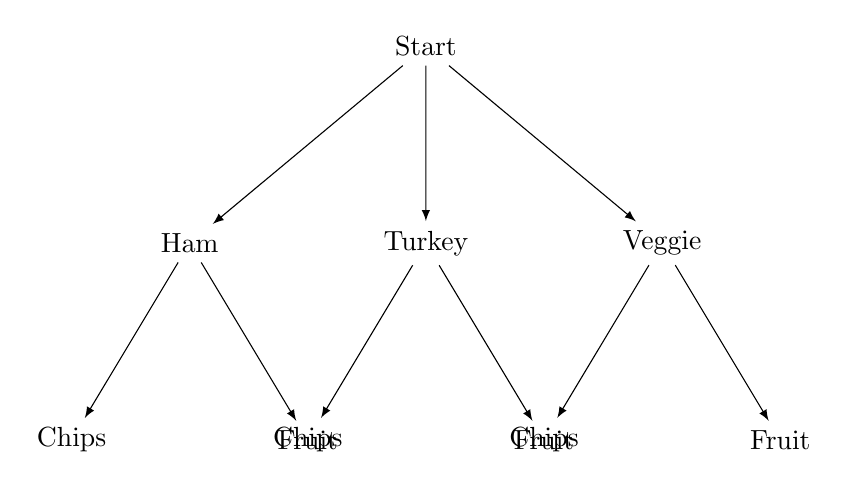
\begin{tikzpicture}[level distance=2.5cm, sibling distance=3cm,
  edge from parent/.style={draw,-latex}]
  \node {Start}
    child { node {Ham}
      child { node {Chips} edge from parent node[left] {} }
      child { node {Fruit} edge from parent node[right] {} }
      edge from parent node[left] {}
    }
    child { node {Turkey}
      child { node {Chips} edge from parent node[left] {} }
      child { node {Fruit} edge from parent node[right] {} }
      edge from parent node[right] {}
    }
    child { node {Veggie}
      child { node {Chips} edge from parent node[left] {} }
      child { node {Fruit} edge from parent node[right] {} }
      edge from parent node[right] {}
    };
\end{tikzpicture}
\end{center}

If each combination is equally likely, what is the probability of getting Turkey with Fruit?
\end{questionText}
\choiceA{$\dfrac{1}{2}$}
\choiceB{$\dfrac{1}{3}$}
\choiceC{$\dfrac{1}{5}$}
\choiceD{$\dfrac{1}{6}$}
\correctAnswer{D}
\explanation{The tree diagram shows $3 \times 2 = 6$ equally likely outcomes. ``Turkey with Fruit'' is $1$ outcome, so $P = \frac{1}{6}$.}
\end{practiceQuestion}

\begin{practiceQuestion}{9-6-q24}{gmc}
\begin{questionText}
The table below shows the products when two spinners are spun. Spinner 1 has sections $\{1, 2, 3\}$ and Spinner 2 has sections $\{2, 4, 6\}$.

\begin{center}
\begin{tabular}{c|ccc}
$\times$ & \textbf{2} & \textbf{4} & \textbf{6} \\
\hline
\textbf{1} & $2$ & $4$ & $6$ \\
\textbf{2} & $4$ & $8$ & $12$ \\
\textbf{3} & $6$ & $12$ & $18$ \\
\end{tabular}
\end{center}

What is the probability that the product is greater than $10$?
\end{questionText}
\choiceA{$\dfrac{1}{9}$}
\choiceB{$\dfrac{2}{9}$}
\choiceC{$\dfrac{1}{3}$}
\choiceD{$\dfrac{4}{9}$}
\correctAnswer{C}
\explanation{Products greater than $10$: $12, 12, 18$ — $3$ outcomes out of $9$ total. $\frac{3}{9} = \frac{1}{3}$.}
\end{practiceQuestion}

% --- Graphical Short Answer Questions (3) ---

\begin{practiceQuestion}{9-6-q25}{gsa}
\begin{questionText}
The table shows all outcomes when a coin is flipped and a spinner with sections $\{1, 2, 3, 4\}$ is spun.

\begin{center}
\begin{tabular}{c|cccc}
 & \textbf{1} & \textbf{2} & \textbf{3} & \textbf{4} \\
\hline
\textbf{H} & H1 & H2 & H3 & H4 \\
\textbf{T} & T1 & T2 & T3 & T4 \\
\end{tabular}
\end{center}

What is the probability of getting tails and a number greater than $2$? Express your answer as a simplified fraction.
\end{questionText}
\correctAnswer{$\frac{1}{4}$}
\explanation{Tails and greater than $2$: T3, T4 — $2$ favorable outcomes out of $8$ total. $\frac{2}{8} = \frac{1}{4}$.}
\end{practiceQuestion}

\begin{practiceQuestion}{9-6-q26}{gsa}
\begin{questionText}
The tree diagram shows outcomes for choosing an appetizer and an entree at a restaurant.

\begin{center}
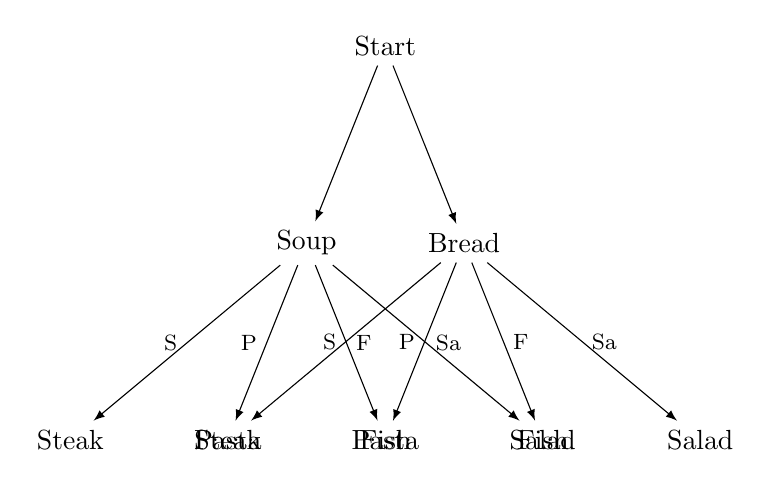
\begin{tikzpicture}[level distance=2.5cm, sibling distance=2cm,
  edge from parent/.style={draw,-latex}]
  \node {Start}
    child { node {Soup}
      child { node {Steak} edge from parent node[left] {\footnotesize S} }
      child { node {Pasta} edge from parent node[left] {\footnotesize P} }
      child { node {Fish} edge from parent node[right] {\footnotesize F} }
      child { node {Salad} edge from parent node[right] {\footnotesize Sa} }
      edge from parent node[left] {}
    }
    child { node {Bread}
      child { node {Steak} edge from parent node[left] {\footnotesize S} }
      child { node {Pasta} edge from parent node[left] {\footnotesize P} }
      child { node {Fish} edge from parent node[right] {\footnotesize F} }
      child { node {Salad} edge from parent node[right] {\footnotesize Sa} }
      edge from parent node[right] {}
    };
\end{tikzpicture}
\end{center}

If each combination is equally likely, what is the probability of choosing Bread as the appetizer and NOT choosing Steak? Express your answer as a simplified fraction.
\end{questionText}
\correctAnswer{$\frac{3}{8}$}
\explanation{Total outcomes: $2 \times 4 = 8$. Bread with something other than Steak: Bread-Pasta, Bread-Fish, Bread-Salad — $3$ outcomes. $\frac{3}{8}$.}
\end{practiceQuestion}

\begin{practiceQuestion}{9-6-q27}{gsa}
\begin{questionText}
The sample space table shows the absolute differences when two number cubes are rolled.

\begin{center}
\begin{tabular}{c|cccccc}
$|\ |$ & \textbf{1} & \textbf{2} & \textbf{3} & \textbf{4} & \textbf{5} & \textbf{6} \\
\hline
\textbf{1} & $0$ & $1$ & $2$ & $3$ & $4$ & $5$ \\
\textbf{2} & $1$ & $0$ & $1$ & $2$ & $3$ & $4$ \\
\textbf{3} & $2$ & $1$ & $0$ & $1$ & $2$ & $3$ \\
\textbf{4} & $3$ & $2$ & $1$ & $0$ & $1$ & $2$ \\
\textbf{5} & $4$ & $3$ & $2$ & $1$ & $0$ & $1$ \\
\textbf{6} & $5$ & $4$ & $3$ & $2$ & $1$ & $0$ \\
\end{tabular}
\end{center}

What is the probability that the absolute difference is $0$ (i.e., both dice show the same number)? Express your answer as a simplified fraction.
\end{questionText}
\correctAnswer{$\frac{1}{6}$}
\explanation{A difference of $0$ means both dice match: $(1,1), (2,2), (3,3), (4,4), (5,5), (6,6)$ — $6$ outcomes out of $36$. $\frac{6}{36} = \frac{1}{6}$.}
\end{practiceQuestion}
